\documentclass[../thesis.tex]{subfiles}

\begin{document}

Η εφαρμογή μας συνοδεύεται από μία ιστοσελίδα που περιέχει συμπληρωματικές πληροφορίες όπως τους όρους χρήσης και την πολιτική απορρήτου, και η οποία επιτρέπει στους χρήστες να δουν τις λεπτομέρειες του λογαριασμού τους αλλά και να διαγράψουν τα αποθηκευμένα στοιχεία τους.
Επομένως, εκτός από τους servers που αναλύσαμε στο κύριο μέρος οι οποίοι είναι απαραίτητοι για τη λειτουργία της εφαρμογής, διαθέτουμε και έναν ακόμα ανεξάρτητο web server που είναι υπεύθυνος για την ιστοσελίδα αυτή.

\bigskip

Ο server χρησιμοποιεί το framework Express.js, το πιο ευρέως διαδεδομένο framework για τη δημιουργία web εφαρμογών μέσω του Node.js.

Οι στατικές σελίδες παρέχονται απευθείας από το Nginx και δεν παρουσιάζουν ιδιαίτερο ενδιαφέρον.
Επομένως, θα αναλύσουμε το μέρος της ιστοσελίδας που είναι δυναμικό, δηλαδή τη σελίδα που εμφανίζει το προφίλ του χρήστη.
Η χρήση του Express.js βασίζεται στο αντικείμενο που κατά σύμβαση ονομάζουμε \texttt{app} το οποίο περιέχει όλο το API του framework, και μέσω του οποίου ορίζουμε τη συμπεριφορά της εφαρμογής.
Το παρακάτω μέρος του κώδικα ορίζει τη συμπεριφορά της εφαρμογής όταν ο χρήστης μεταβεί στη σελίδα του προφίλ του (GET request στο relative URL \texttt{/profile}).
Εφόσον η σελίδα αυτή δεν είναι ίδια για τον κάθε χρήστη, ο server χρειάζεται να ξέρει την ταυτότητα του ατόμου προκειμένου να στείλει τη σωστή σελίδα με τα στοιχεία του.
Έτσι ο server πραγματοποιεί πρώτα το authentication του χρήστη, και αφού διαπιστώσει την ταυτότητά του προσπελάζει τη βάση δεδομένων για να συμπληρώσει τη σελίδα με τα κατάλληλα στοιχεία\footnote{Η συμπλήρωση του HTML αρχείου με τα κατάλληλα στοιχεία γίνεται μέσω της EJS, μίας απλής γλώσσας templating για HTML}.
Όταν ο server ταυτοποιήσει έναν χρήστη αποθηκεύει τον ΑΜ του στο αντίστοιχο session έτσι ώστε μελλοντικά αιτήματα στη σελίδα προφίλ να μην απαιτούν ξανά την ταυτοποίηση του χρήση, τουλάχιστον μέχρι ο χρήστης να τερματίσει το session κλείνοντας τον browser του.

\begin{codeblock}
  const app = express();

  app.get("/profile", async (req, res) => {
    if (!req.session.userId) {
      res.redirect("/auth");
      return;
    }
    let user = await getUser(req.session.userId);
    if (!user) {
      res.status(500).redirect("/");
      return;
    }

    res.render("profile", {
      id: user.id,
      name: user.full_name,
      cars: user.cars,
      ratings_count: user.ratings_count,
      ratings_sum: user.ratings_sum,
      picture: user.picture,
    });
  });
\end{codeblock}

Έτσι λοιπόν βλέπουμε ότι όταν ο χρήστης μεταβεί στη σελίδα \texttt{profile} ελέγχουμε αρχικά αν υπάρχει ήδη session, και αν όχι τότε οδηγούμε τον χρήστη στη σελίδα ταυτοποίησης \texttt{auth}.
Αν ο χρήστης είναι ταυτοποιημένος τότε μέσω της \texttt{getUser} διαβάζουμε όλα τα στοιχεία του από τη βάση, και έπειτα στέλνουμε τη συμπληρωμένη σελίδα προφίλ μέσω της συνάρτησης \texttt{render}.

\bigskip

Ακολουθεί ο χειρισμός του authentication:

\begin{codeblock}{typescript}{website.ts}
  const myIssuer = await Issuer.discover(env.ISSUER);

  const oidcClient = new myIssuer.Client({
    client_id: env.WEB_CLIENT_ID,
    client_secret: env.WEB_CLIENT_SECRET,
    redirect_uris: [env.WEB_REDIRECT_URI],
    response_types: ["code"],
  });

  app.get("/auth", (req, res) => {
    req.session.codeVerifier = generators.codeVerifier();
    const code_challenge = generators.codeChallenge(req.session.codeVerifier);
    const authUrl =
      oidcClient.authorizationUrl({
        scope: "openid profile email",
        code_challenge: code_challenge,
        code_challenge_method: "S256",
      }) + "&kc_idp_hint=saml";
    res.redirect(authUrl);
  });

  app.get("/auth/cb", async (req, res) => {
    const params = oidcClient.callbackParams(req);
    try {
      const tokenSet = await oidcClient.callback(env.WEB_REDIRECT_URI, params, {
        code_verifier: req.session.codeVerifier,
      });
      if (!tokenSet.claims().id) {
        res.status(401).send();
        return;
      }
      req.session.idToken = tokenSet.id_token;
      req.session.userId = tokenSet.claims().id;
      res.redirect("/profile");
    } catch (error) {
      res.status(401).send();
    }
  });
\end{codeblock}

Αρχικά δημιουργούμε τον OpenID Client που θα είναι μέρος του server μας εισάγοντας τα στοιχεία που ορίσαμε κατά την εγγραφή στον OpenID Provider του Keycloak.
Όπως είδαμε προηγουμένως, όταν απαιτείται η ταυτοποίηση ενός χρήστη μεταβαίνουμε στο route \texttt{/auth}.
Από εκεί κάνουμε redirect τον χρήστη στο URL του provider όπου θα πραγματοποιηθεί η ταυτοποίηση, περνώντας το λεγόμενο code challenge που είναι κρίσιμο για τη λειτουργία του PKCE.
Μόλις η ταυτοποίηση ολοκληρωθεί, ο OpenID Provider ανακατευθύνει τον χρήστη στο URL \texttt{/auth/cb} της ιστοσελίδας μας, συμπεριλαμβάνοντας μία σειρά από παραμέτρους στο URL, και ο server μπορεί χρησιμοποιώντας αυτές τις παραμέτρους να ζητήσει το ID token του χρήστη μέσω ενός POST request στον OpenID provider.
Το ID token αποθηκεύεται στο session του χρήστη, και ο χρήστης μεταβαίνει τελικά στη σελίδα προφίλ του.

Τέλος, έχουμε τις δύο δράσεις της σελίδας προφίλ, την αποσύνδεση και τη διαγραφή λογαριασμού:

\begin{codeblock}{typescript}{website.ts}
  app.post("/profile/logout", (req, res) => {
    const logoutUrl = oidcClient.endSessionUrl({
      post_logout_redirect_uri: env.WEB_LOGOUT_REDIRECT_URI,
      id_token_hint: req.session.idToken,
    });
    res.redirect(logoutUrl);
    req.session.destroy((err) => {
      if (err) loggerMain.error(err);
    });
  });

  app.post("/profile/delete", async (req, res) => {
    if (!req.session.userId) {
      res.status(401).send();
      return;
    }
    await removeUser(req.session.userId);
    res.redirect("/profile/logout");
  });
\end{codeblock}

Κατά την αποσύνδεση, ο server απλά οδηγεί τον χρήστη στο κατάλληλο URL του OpenID Provider το οποίο θα τον αποσυνδέσει από τον λογαριασμό του, και έπειτα καταστρέφει το αντίστοιχο session.
Αντίστοιχα όταν ο χρήστης πατάει του κουμπί διαγραφής τότε διαγράφουμε τον λογαριασμό του από τη βάση δεδομένων και προχωράμε στην αποσύνδεσή του.

\bigskip

Για την υλοποίηση των sessions χρησιμοποιούμε τη NoSQL βάση δεδομένων Redis.
Το κάθε session αποθηκεύεται ως ένα key-value pair, με το session ID να χρησιμοποιείται ως key και το αντίστοιχο session cookie ως value.

Μία σημαντική λεπτομέρεια που πρέπει να τονίσουμε είναι το attribute SameSite που θέτουμε ως "Lax" στo session cookie.
Το attribute αυτό πληροφορεί τον browser του χρήστη για το πως να χειριστεί την αποστολή του συγκεκριμένου cookie στην περίπτωση request που προέρχεται από διαφορετική ιστοσελίδα.
Συγκεκριμένα, η ρύθμιση Lax σημαίνει ότι αν μία τυχαία ιστοσελίδα προσπαθήσει να στείλει ένα POST request στην ιστοσελίδα μας, τότε ο browser \textit{δεν} θα μεταφέρει μαζί με το request το session cookie του χρήστη.

Το παραπάνω αποτελεί μέθοδο προστασίας έναντι επιθέσεων μέσω cross-site request forgery, και χρησιμοποιείται συγκεκριμένα για τη δράση του κουμπιού διαγραφής λογαριασμού.
Το πάτημα το κουμπιού διαγραφής στέλνει απλά ένα POST request στο κατάλληλο route της εφαρμογής το οποίο εκτελεί τη διαγραφή του χρήστη από τη βάση δεδομένων.
Αν ο χρήστης επισκεφτεί μία ξένη κακόβουλη ιστοσελίδα (cross-site) τότε αυτή μπορεί πολύ εύκολα να στείλει το ίδιο ακριβώς request εκ μέρους του, και αν ο browser συμπεριλάβει το session cookie με αυτό το request τότε η ιστοσελίδα μπορεί να διαγράψει τον λογαριασμό του χρήστη εν αγνοία του.
Το πρόβλημα λύνεται με τον ορισμό του cookie ως Lax, καθώς σε αυτή την περίπτωση ο browser του χρήστη δεν θα στείλει το αντίστοιχο session cookie με το POST request, και επομένως δε θα πραγματοποιήσει την καταστροφική πράξη.

\begin{codeblock}{typescript}{website.ts}
  declare module "express-session" {
    export interface SessionData {
      codeVerifier: string;
      idToken: string;
      userId: string;
    }
  }

  let redisClient = createClient();
  redisClient.connect().catch(loggerMain.error);
  let redisStore = new RedisStore({ client: redisClient, prefix: "ridehailing" });

  app.use(
    session({
      store: redisStore,
      secret: env.SESSION_SECRET,
      resave: false,
      saveUninitialized: false,
      cookie: { secure: true, httpOnly: true, sameSite: "lax" },
    })
  );
\end{codeblock}

\begin{figure}
  \centering
  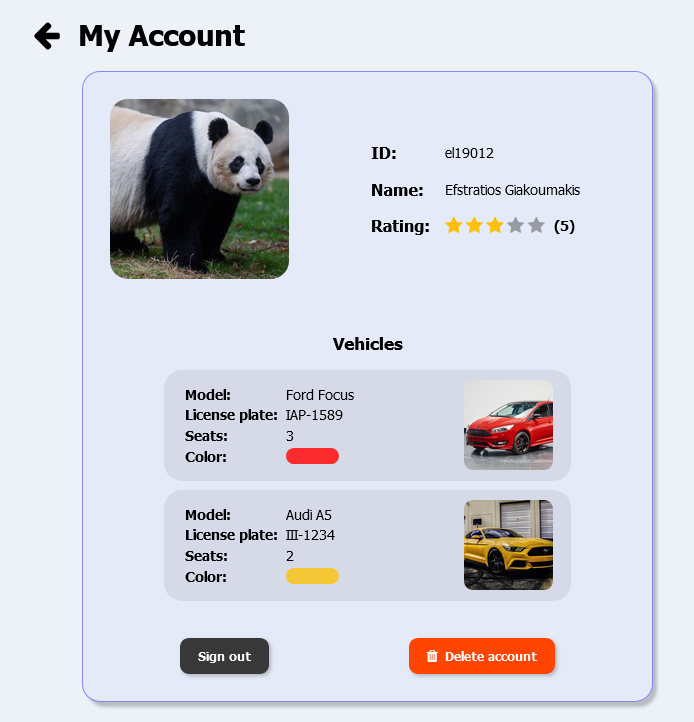
\includegraphics[width=\textwidth]{website.png}
  \caption{Η σελίδα προφίλ όπου εμφανίζονται όλα τα στοιχεία ενός χρήστη. Το URL της ιστοσελίδας είναι \url{https://ntua-ridehailing.dslab.ece.ntua.gr/profile}}
\end{figure}

\end{document}